\section{高性能模式}
这个文档和伴随的\href{https://github.com/tensorflow/benchmarks/tree/master/scripts/tf_cnn_benchmarks}{脚本}详细介绍了日结构建大规模的针对多系统类型和网络拓扑模型的大规模模型。在这个文档中的技术使用一些低级的TensorFlow Python原语。在将来这些技术中的一些江北整合进高级API。
\subsection{输入pipline}
在\href{https://www.tensorflow.org/performance/performance_guide}{Performance Guide}中解释了如何确定可能的输入pipeline问题和最优的实践。我们发现使用\href{https://www.tensorflow.org/api_docs/python/tf/FIFOQueue}{tf.FIFOQueue}和 \href{https://www.tensorflow.org/api_docs/python/tf/train/queue_runner}{tf.train.queue\_runner} 在每秒处理大型输入(像训练ImageNet的\href{http://papers.nips.cc/paper/4824-imagenet-classification-with-deep-convolutional-neural-networks.pdf}{AlexNet})和样本的时候不能跑满多个当前常用的GPU。这是因为使用Python线程作为实现。Python线程的开支太大。

另一个实现方案是我们在TensorFlow上用本地并行构建一个输入pipeline,我们在 \href{https://github.com/tensorflow/benchmarks/tree/master/scripts/tf_cnn_benchmarks}{脚本}中实现了这个方法。w我们的实现由三个stage组成:
\begin{itemize}
\item I/O读:选择从磁盘中读取图像文件
\item 图像处理:解码图像记录为图像,处理组织他们为一个mini-batch
\item CPU-to-GPU数据转换。从CPU转换图像到GPU
\end{itemize}
每一个的主要部分结合其他部分使用data\_flow\_ops.StringArea,StagingArea(类似tf.FIFOQueue)。不同的是StagingArea不保证FIFO的孙旭,但是提供简单的函数,结合其他的stage在CPU和GPU上平行执行。分开输入pipeline为三个stage,操作独立并行运行是规模化的充分利用的多核环境。下面的章节详细的介绍了data\_flow\_ops.String。
\subsection{并行化I/O读取}
data\_flow\_ops.RecordInput用于从磁盘上并行化读取。给定一个输入文件表示TFRecord,RecordInput持续使用后台线程读取记录。记录被放在他自己的打的内部线程池单后在至少一半容量的时候载入,产生输出tensor。

这个操作自己的内部的线层被小号最小CPU的I/O时间决定,这允许模型剩下的部分平稳运行。

\subsection{并行化图像处理}
在图像从RecordInput读取后他们被作为tensor传递给图像处理pipeline。为了确保图像处理pipeline容易解释,假设输入pipeline是每256大小的批有8GPU。

并行的时候有256个记录被单独处理。这在图上开启了256个独立的RecordInput读op。每个读op跟着一些用于图像处理的操作在并行运行时独立执行。图像预处理操作包含想图像解码,变形和变换大小。

当图像被处理的时候他们每批32被连接进入8个tensor.相比于使用\href{https://www.tensorflow.org/api_docs/python/tf/concat}{tf.concat}达到这个目的,作为一个单独的操作实现等待所有的输入在连接他们在一起之前被准备好,\href{https://www.tensorflow.org/api_docs/python/tf/parallel_stack}{tf.parallel\_stack}被使用。\href{https://www.tensorflow.org/api_docs/python/tf/parallel_stack}{tf.parallel\_stack}分配一个没有初始化的tensor作为输出,每个输入tensor被写入,他的设计输出部分的tensor,只要输入是可用的。

当所有的输入完成后,输出tensor沿着图传递。这结合所有输入tensor产生的长尾隐藏内存占有。

\subsection{并行化CPU到GPU数据转化}
继续这个假设,目标是8GPU每批大小256(每个GPU32).当输入图像通过CPU处理和连接,我们每批大小32有8个tensor。

TensorFlow使得来自于一个设备的tensor能在其他任何设备上使用。tensor实际使用之前在设备之间复制运行调度。然而,如果复制不能及时完成,需要这些tensor的计算将停止导致性能下降。

在这个实现中data\_flow\_ops.StagingArea用于明确的在并行处理中调度。结果时当计算从GPU上开始时。所有的tensor已经可用。

\subsection{软件pipeline}
结合所有由不同处理器驱动的stage能力,data\_flow\_ops.StagingArea用在他们之间因此他们在并行处理中运行。StagingArea是类似\href{https://www.tensorflow.org/api_docs/python/tf/FIFOQueue}{tf.FIFOQueue}一个队列的操作,它提供简单的函数在CPU和GPU上执行。

在模型开始运行所有的stages之前,输入pipeline stage被warmed up到到主要的staging缓存。在每个运行步,一些数据在每个stage开始从staging buffer读取,一个被推到结尾。

例如:如果有三个stage A,B,C,有两个staging在S1和S2之间,warmi up中,我们运行:
\begin{lstlisting}[language=Bash]
Warm up:
Step 1: A0
Step 2: A1  B0

Actual execution:
Step 3: A2  B1  C0
Step 4: A3  B2  C1
Step 5: A4  B3  C2
\end{lstlisting}
在warm up后,S1和S2有一些数据,实际执行的每一步,一些数据从每个stageing area被小号,一些被添加到另一个集合。
使用这种机制的好处:
\begin{itemize}
	\item 所有的stages都是非模块的,因为stage area总有一些数据在warm up后
	\item 每个stage能并行运行,因此他们可以立即开始
	\item 在固定内存的staging buffer。我们将有一些额外的数据
	\item 仅仅单个session.run()调用需要运行所有步骤的stage,使得探测和吊事更容易
\end{itemize}
\subsection{构建高性能模型的最佳实践}
手机下面一些额外的联系可以提高性能增加模型的灵活度。
\subsection{用NHWC和NCHW构建模型}
大多数的CNN使用的TensorFlow操作支持NHWC和NCHW数据核实。在GPU上,NCHW更快,但是在CPU上,NHWC有时候更快。

构建一个模型支持两种数据格式保证模型灵活和忽略平台优化操作的能力。CNN中多数TensorFlow操作支持NHWC和NCHW数据格式。基准脚本支持NCHW和NHWC。NCHW应该总是当在GPU上训练的时候用。NHWC有时在CPU上运行更快。一个灵活的模型可以再GPU上用NCHW训练在CPU上用NHWC上结合训练的权重推理。
\subsection{使用融合的Batch-Normalization}
一个TensorFlow默认的BN作为组件操作被实现。这是非常常见的,但是进仓导致次优的性能。一个可选方案是用融合在GPU上有更高性能的normalization。下面的例子是使用\href{https://www.tensorflow.org/api_docs/python/tf/contrib/layers/batch_norm}{tf.contrib.layers.batch\_norm}实现融合的BN。
\begin{lstlisting}[language=Python]
bn = tf.contrib.layers.batch_norm(
          input_layer, fused=True, data_format='NCHW'
          scope=scope)
\end{lstlisting}
\subsection{变量分布和梯度聚合}
在训练中,训练的变量值私用聚合的梯度和delta更新训练变量。在基准测试脚本中,我们展示了灵活和通常目的的TensorFlow原语,一个从该性能分布和聚合方案的多种构建。
变量分布和聚合的例子包含在脚本中:
\begin{itemize}
	\item parameter\_server 每个训练模型的复制从参数服务器读取变量,单独的更新变量。当每个模型需要变量的时候,他们被通过标准的隐含复制由TensorFlow运行环境添加。示例\href{https://github.com/tensorflow/benchmarks/tree/master/scripts/tf_cnn_benchmarks}{脚本}参数在本地训练使用这个方法,分布的同步训练,分布的一步训练。
	\item replicated 在每个GPU上放置完全相同的的复制的变量。前向计算和后向计算可以立即开始作为变量数据。梯度通过所有的GPU累积,聚合在一起用于每个GPU的肤质变量保证他们同步。
	\item distributed\_replicated 在每个GPU上沿着主要的参数服务器放置完全相同的训练参数,当变量数据可用的时候前向后向计算立即开始。梯度通过在服务器上的GPU累积然后每个服务器聚合梯度用于主要的copy。在所有的worker做这件事后,每个worker更新他从主机复制来的参数
\end{itemize}
下面是额外的关于每个方法的详细信息。
\subsection{参数服务器变量}
多数情况下可训练的变量在TensorFlow模型中管理是以参数服务器模式。

在一个分布式系统,每个worker处理同一model的运行,每个参数服务器处理自己的住的从主机(master)复制过来的变量。当worker需要从参数服务器获得变量的时候。它直接访问。在TensorFlow运行环境中添加隐含的复制到图上确保变量需要的时候的值在计算设备之间可用。当一个梯度在worker上计算的时候,它发送到参数服务器自己的变量,对应的优化器用于更新变量。

有一些技术提高吞吐率:
\begin{itemize}
    \item 变量基于他的大小在参数服务器间分散,用于负载均衡
    \item 每个worker有多个GPU,梯度在GPU上累积单个聚合梯度发送到参数服务器。这减少的网络带宽和参数服务器的work数量
\end{itemize}
对普通的两个worker,一个常见模式是异步更新,这里每个worker不用和他和其他的worker同步更新各自从master得到的参数。我们展示这是一个公平的方法在worker之间介绍同步因此对于所有的worker更新在下一步能开始前完成。

参数服务器方法也能用于本地训练,在这种情况下扩山从master负载来的变量到哥哥服务器,他们技能在CPU上可能在可用的GPU上运行。

因为这个开启的简单性质,这个架构已经在在社区中流行起来了。

模式可能通过传递--variable\_update=parameter\_server用在脚本中。
\begin{figure}
	\centering
	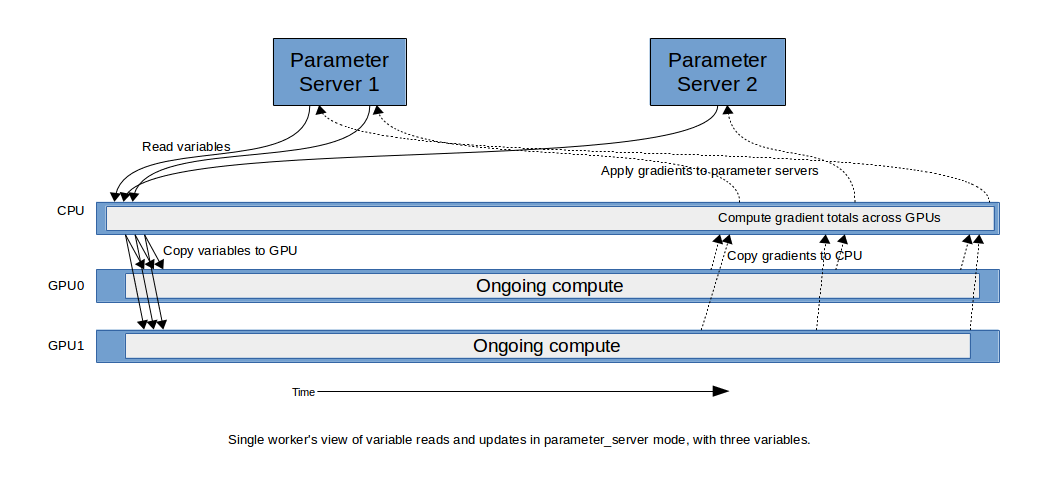
\includegraphics[scale=0.5]{perf_parameter_server_mode_doc.png}
\end{figure}
\subsection{复制的变量}
在这个设计中,每个在server上的GPU有自己的复制的变量。值通过应用完整的局和提取到每个GPU的复制变量保持同步。

变量和数据在训练开始的时候是可用的,因此钱想传递训练可以立即开始。梯度通过device聚合,完整的聚合的梯度是应用在每个本地复制。
梯度聚合通过server扩山到server有不同的方法:
\begin{itemize}
	\item 使用标准的TensorFlow操作聚合在一个单独的device(CPU或者GPU)然后复制它回到所有的GPUs
	\item 使用NVIDIANCCL,下面的NCCL章节描述。
\end{itemize}
这个模式可以通过传递--variable\_update=replicated用在脚本中。
\subsection{在分布式系统上训练时复制变量}
对于变量的复制方法可能被扩展到分布式训练。一个处理这样工作的方法是replicated mode:完全通过集群聚合梯度然后应用他们到每个本地复制变量。这在这个脚本的将来版本也许会显示,脚本呈现一个不同的变量,描述。

在这个模式,额外的每个GPU的复制变量,master的复制存储在村塾服务器。正如复制模式,训练可以用本地的复制的变量立即开始。

当权重的梯度可用的时候,他们送回参数服务器所有的本地复制被更新:
\begin{enumerate}
	\item 所有从同一个worker来的梯度被聚集在一起
	\item 从每个worker聚集的梯度被发送到参数服务器拥有的变量,这里制定的优化器用于更新master变量的复制
	\item 每个worker更新它从master复制的变量。在例程模型,这集合cross-replica做等待所有workers完成更新变量,仅仅在所有复制的障碍被释放后获取新的变量。当一个对所有变量的复制完成后,这标记训练的末端,下一步训练可以开始。
\end{enumerate}
尽管这听起来类似使用参数服务器的标准,但是性能进场更好。很可能是应为计算没有延迟,大量复制的梯度的时延可能通过之后的计算曾被隐
这个模式可以传递参数--variable\_update=distributed\_replicated用于脚本。
\begin{figure}[H]
	\centering
	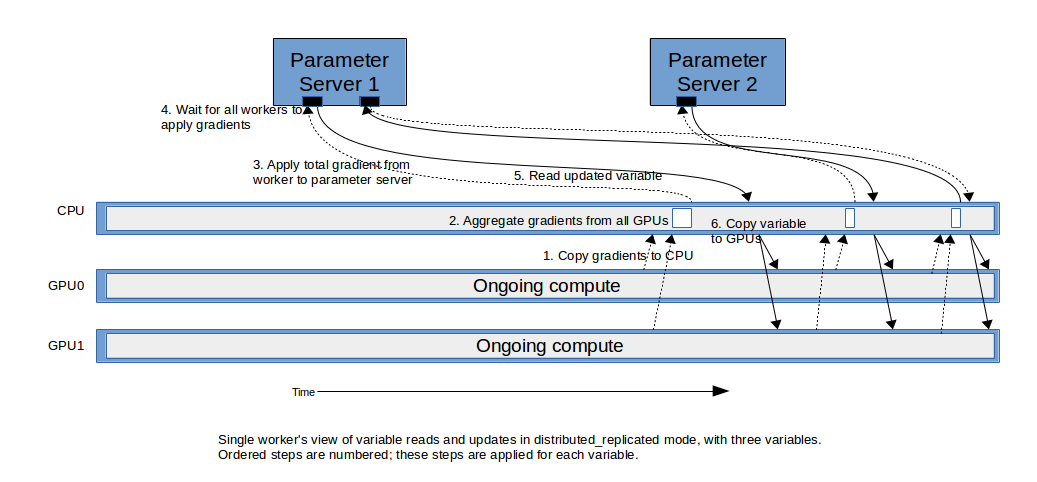
\includegraphics[scale=0.5]{perf_distributed_replicated_mode_doc.png}
\end{figure}
\subsection{NCCL}
为了广播变量在同一机器上通过不同的GPU聚合梯度梯度,我们可以使用默认的TensorFlow隐藏的复制机制。

然而,我们可以使用选项NCCL(\href{https://www.tensorflow.org/api_docs/python/tf/contrib/nccl}{tf.contrib.nccl})。NCCL是NVIDIA一个能在不同的GPU上可以高效广播和聚合数据库。它在每个GPU上调度一个cooperatting核心了解基础硬件拓扑下的最佳利用。这可信使用一个GPU的SM。

在我们的试验中,我们通过NCLL展示经常比本身有更快的数据聚合。我们的假设是隐含的复制隐含的基本的free因此他们能在GPU上复制引擎,只要时延能通过主要的计算本身隐藏。尽管NCLL可以更快的转换数据,接受一个SM,给基于L2cache添加更多压力。我们的结果显示8GPU,NCLL载入更好的性能。然而很少的GPU,隐含的复制性能更好。
\subsection{Staged变量}
我们进一步介绍一个staged变量模式,这里我们用staging area到变量读和他们的更新。类似输入pipeline的软件的pipelining,这可以隐藏数据复制时延。如果计算时间花费被复制和聚合更长,复制它本身变得essentially free。

缺点是所有的权重从之前训练步骤读取。因此它不同于SGD算法。但是它能通过掉着那个学习率和其它草参数可能改善收敛。

\subsection{执行脚本}
这个章节列出命令行参数的核心和有一些基本的执行主要脚本的例子( \href{https://github.com/tensorflow/benchmarks/tree/master/scripts/tf_cnn_benchmarks/tf_cnn_benchmarks.py}{tf\_cnn\_benchmarks.py})
\begin{quote}
	\textbf{注意:}\emph{tf\_cc\_benchmarks.py用在TensorFlow 1.1之后引入的force\_gpu\_campatible,知道TensorFlow 1.2被从源代码被释放被建议。}
\end{quote}
\subsection{基本的命令行参数}
\begin{itemize}
	\item model:模型使用。如resnet50,inception3,vgg16和alexnet
	\item num\_gpus:使用GPU的数量
	\item data\_dir:处理数据的路径。如果没有设置,中和数据被使用。用imagenet数据这些\href{https://github.com/tensorflow/models/tree/master/inception#getting-started}{说明}作为起点。
	\item batch\_size:每个GPU的批的尺寸
	\item variable\_update:管理变量的方法:parameter\_server ,replicated, distributed\_replicated, independent
	\item local\_parameter\_device:用作参数服务器的设备:CPU或者GPU
\end{itemize}
单个实例的例子
\begin{lstlisting}[language=Python]
# VGG16 training ImageNet with 8 GPUs using arguments that optimize for
# Google Compute Engine.
python tf_cnn_benchmarks.py --local_parameter_device=cpu --num_gpus=8 \
--batch_size=32 --model=vgg16 --data_dir=/home/ubuntu/imagenet/train \
--variable_update=parameter_server --nodistortions

# VGG16 training synthetic ImageNet data with 8 GPUs using arguments that
# optimize for the NVIDIA DGX-1.
python tf_cnn_benchmarks.py --local_parameter_device=gpu --num_gpus=8 \
--batch_size=64 --model=vgg16 --variable_update=replicated --use_nccl=True

# VGG16 training ImageNet data with 8 GPUs using arguments that optimize for
# Amazon EC2.
python tf_cnn_benchmarks.py --local_parameter_device=gpu --num_gpus=8 \
--batch_size=64 --model=vgg16 --variable_update=parameter_server

# ResNet-50 training ImageNet data with 8 GPUs using arguments that optimize for
# Amazon EC2.
python tf_cnn_benchmarks.py --local_parameter_device=gpu --num_gpus=8 \
--batch_size=64 --model=resnet50 --variable_update=replicated --use_nccl=False
\end{lstlisting}
\subsection{分布式的命令行参数}
\begin{itemize}
	\item ps\_host:逗号分隔的主机用作参数服务器,格式为<host>:port,例如10.0.0.2:50000
	\item worker\_hosts:逗号分隔的主机用作worker,格式<host>:port,例如10.0.0.2:50001
	\item task\_index:在ps\_hosts或者worker\_hosts开始的主机索引
	\item job\_name:输入job,例如ps或者worker 
\end{itemize}
\subsection{分布式的例子}
下面是一个在两台主机上训练ResNet-50的例子host\_0(10.0.0.1)和host\_1(10.0.0.2)使用中和数据的例子,用通过传递--data\_dir参数传递真实数据。
\begin{lstlisting}[language=Python]
# Run the following commands on host_0 (10.0.0.1):
python tf_cnn_benchmarks.py --local_parameter_device=gpu --num_gpus=8 \
--batch_size=64 --model=resnet50 --variable_update=distributed_replicated \
--job_name=worker --ps_hosts=10.0.0.1:50000,10.0.0.2:50000 \
--worker_hosts=10.0.0.1:50001,10.0.0.2:50001 --task_index=0

python tf_cnn_benchmarks.py --local_parameter_device=gpu --num_gpus=8 \
--batch_size=64 --model=resnet50 --variable_update=distributed_replicated \
--job_name=ps --ps_hosts=10.0.0.1:50000,10.0.0.2:50000 \
--worker_hosts=10.0.0.1:50001,10.0.0.2:50001 --task_index=0

# Run the following commands on host_1 (10.0.0.2):
python tf_cnn_benchmarks.py --local_parameter_device=gpu --num_gpus=8 \
--batch_size=64 --model=resnet50 --variable_update=distributed_replicated \
--job_name=worker --ps_hosts=10.0.0.1:50000,10.0.0.2:50000 \
--worker_hosts=10.0.0.1:50001,10.0.0.2:50001 --task_index=1

python tf_cnn_benchmarks.py --local_parameter_device=gpu --num_gpus=8 \
--batch_size=64 --model=resnet50 --variable_update=distributed_replicated \
--job_name=ps --ps_hosts=10.0.0.1:50000,10.0.0.2:50000 \
--worker_hosts=10.0.0.1:50001,10.0.0.2:50001 --task_index=1
\end{lstlisting}














